\chapter{Background\label{ch:background}}

Research in the field of \glspl{dl}\index{Digital Libraries} has been going on for over two decades. The mid 1990s, in particular, saw the emergence of a number of government funded projects \citep{Griffin1998},   conferences \citep{Adam1995}, technical committees \citep{DCMI1999,Lorist2001}⁠ and workshops \citep{Dempsey1996,Lagoze1996}⁠, specifically set up to foster formal research in the field of \glspl{dl}. The rapid technological advances and, more specifically, Web technologies have resulted in a number of different \gls{dls} frameworks, conceptual models, architectural designs and \gls{dl}\index{Digital Libraries} software tools. The variation in the designs can largely be attributed to the different design goals and corresponding specific problems that the solutions were aimed to address.

This chapter is organised as follows. Section~\ref{sec:background:digital-libraries} presents an overview of \glspl{dl}, including definitions and sample application domains; Section~\ref{sec:background:fundamental-concepts} introduces fundamental key concepts behind \glspl{dl}; Section~\ref{sec:background:reference-models-frameworks} is a discussion of pioneering work on some proposed frameworks and reference models that have been applied to the implementation of \gls{dls}; Section~\ref{sec:background:digital-libraries-software} presents related work through a discussion of some popular \gls{floss} tools used for managing digital collections; Section~\ref{sec:background:simple-architectures} broadly discusses designs whose successes are hinged on simplicity; Section~\ref{sec:background:data-storage-architectures} discusses some commonly used storage solutions; and finally Section~\ref{sec:background:software-design-decisions} presents two prominent methods used to capture software design decisions.
%Section~\ref{sec:background:software-design-decisions} more generally discusses how contemporary software decision decisions are elicited.

% subsections
\section{Digital Libraries}\index{Digital Libraries}
\label{sec:background:digital-libraries}

\subsection{Definitions}
\label{sec:background:digital-libraries:definitions}

The field of \glspl{dl} \index{Digital Libraries} is a multidisciplinary field that comprises
disciplines such as data management, digital curation, document management,
information management, information retrieval and library sciences. Fox et al.
\citep{Fox1995} outline the varying impressions of \glspl{dl} \index{Digital Libraries} from
persons
in different disciplines and adopt a pragmatic approach of embracing the
different definitions. They further acknowledge the metaphor of the traditional
library as empowering and recognise the importance of knowledge systems that
have evolved as a result. Arms \citep[see][chap. 1]{Arms2000}⁠ provides an
informal definition by viewing a \gls{dl} index{Digital Libraries} as a well organised, managed
network-accessible collection of information---with associated services.

%Nice block diagram on link below...
%http://crd-legacy.lbl.gov/~kewu/ps/LBNL-1677E.pdf

In an attempt to overcome the complex nature of \glspl{dl}, Gon\c{c}alves et
al. \citep{Gonccalves2004}⁠ define a \gls{dl}, using formal methods, by
constructively defining a minimal set of components that make up a \gls{dl}. The set-oriented and functional mathematical formal basis of their
approach facilitates the precise definition of each component as functional
compositions.

The European Union co-funded DELOS\index{DELOS} Network of Excellence on \glspl{dl}
working group proposed a reference model and drafted The \gls{dl}
Manifesto with the aim of setting the foundations and identifying concepts
within the universe of \glspl{dl} \index{Digital Libraries} \citep{Candela2007a}. The DELOS \gls{dl} index{Digital Libraries} reference model envisages a \gls{dl} index{Digital Libraries} universe as a complex
framework and tool having no logical, conceptual, physical, temporal or personal
borders or barriers on information. A \gls{dl} index{Digital Libraries} is perceived as an
evolving organisation that comes into existence through a series of development
steps that bring together all the necessary constituents, each corresponding to
three different levels of conceptualisation of the universe of \glspl{dl}
\citep{Candela2007}⁠. The DELOS \gls{dl} index{Digital Libraries} reference model is discussed in
depth in Section~\ref{sec:background:reference-models-frameworks:delos}.

\subsection{Application domains}
\label{sec:background:digital-libraries:application-domains}

The use of \glspl{dl} \index{Digital Libraries} has become widespread mainly due to the significant
technological advances that have been taking place since the 1990s. The advent
of the Internet has particularly influenced this widespread use. There are
various application domains in which \glspl{dl} \index{Digital Libraries} are used and researchers
are continuously coming up with innovative ways of increasing the footprint of
\gls{dl} index{Digital Libraries} usage. 

Academic institutions are increasingly setting up institutional repositories to
facilitate easy access to research output. \glspl{dl} \index{Digital Libraries} play a vital role
by ensuring that intellectual output is collected, managed, preserved and later
accessed efficiently and effectively. Figure~\ref{fig:background:digital-libraries:zm-cbu-repository} is an illustration of
an institutional repository system---a full text open access institution
repository of the Copperbelt
University\footnote{\url{http://dspace.cbu.ac.zm:8080/jspui}}.

\begin{figure}
 %\begin{center}
 \centering
  \framebox[\textwidth]{%
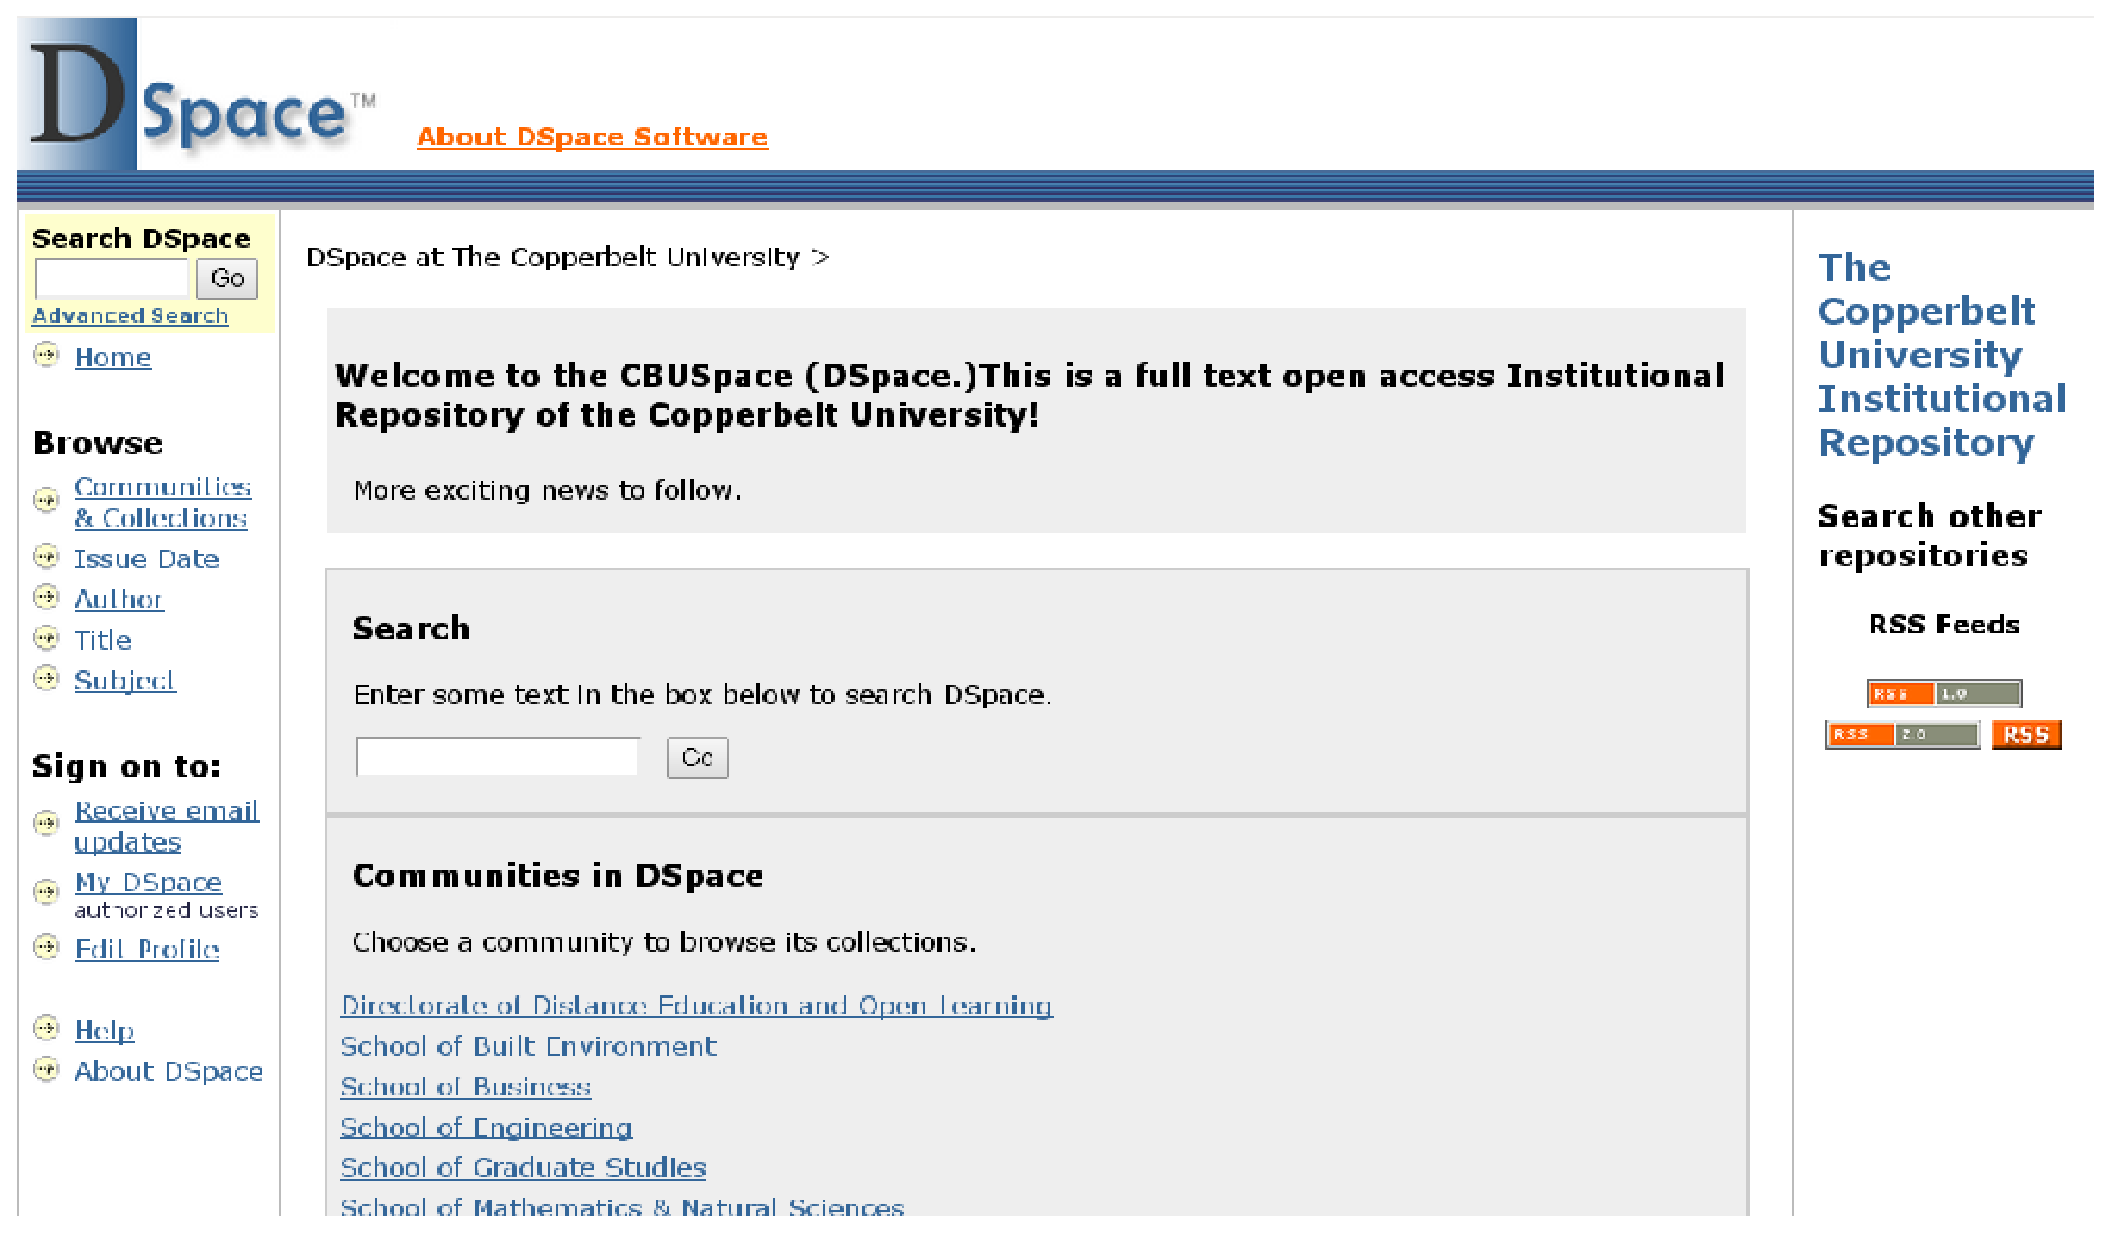
\includegraphics[width=0.95\textwidth]{chapter02/figures/zm-cbu-repository.eps}
  }%
  \caption{Screenshot showing the Copperbelt University institution repository}
  \label{fig:background:digital-libraries:zm-cbu-repository}
 %\end{center}
\end{figure}

Cultural heritage organisations are increasingly digitising historical artifacts
in a quest to display them online to a much wider audience. In light of this,
\glspl{dls} \index{Digital Library System} are being developed to enable easy access to this
information. Figure~\ref{fig:background:digital-libraries:uct-digital-lloydbleekcollection} is a
screen snapshot of the Digital Bleek and Lloyd
Collection\footnote{\url{http://lloydbleekcollection.cs.uct.ac.za}}\index{Bleek\& Lloyd}, which is a
digital collection of historical artifacts that document the culture and
language of the \textbar Xam and !Kun groups of Bushman people of Southern
Africa.

\begin{figure}
 %\begin{center}
  \centering
  \framebox[\textwidth]{%

\includegraphics[width=0.95\textwidth]{%
chapter02/figures/uct-digital-lloydbleekcollection.eps}%
}%
\caption{Screenshot showing the digital Bleek\& Lloyd collection}
\label{fig:background:digital-libraries:uct-digital-lloydbleekcollection}
% \end{center}
\end{figure}


There has also been an increasing number of large scale archival projects that
have been initiated to preserve human knowledge and provide free access to vital
information \citep{Hart1992}.

\begin{figure}
 %\begin{center}
 \centering
  \framebox[\textwidth]{%
  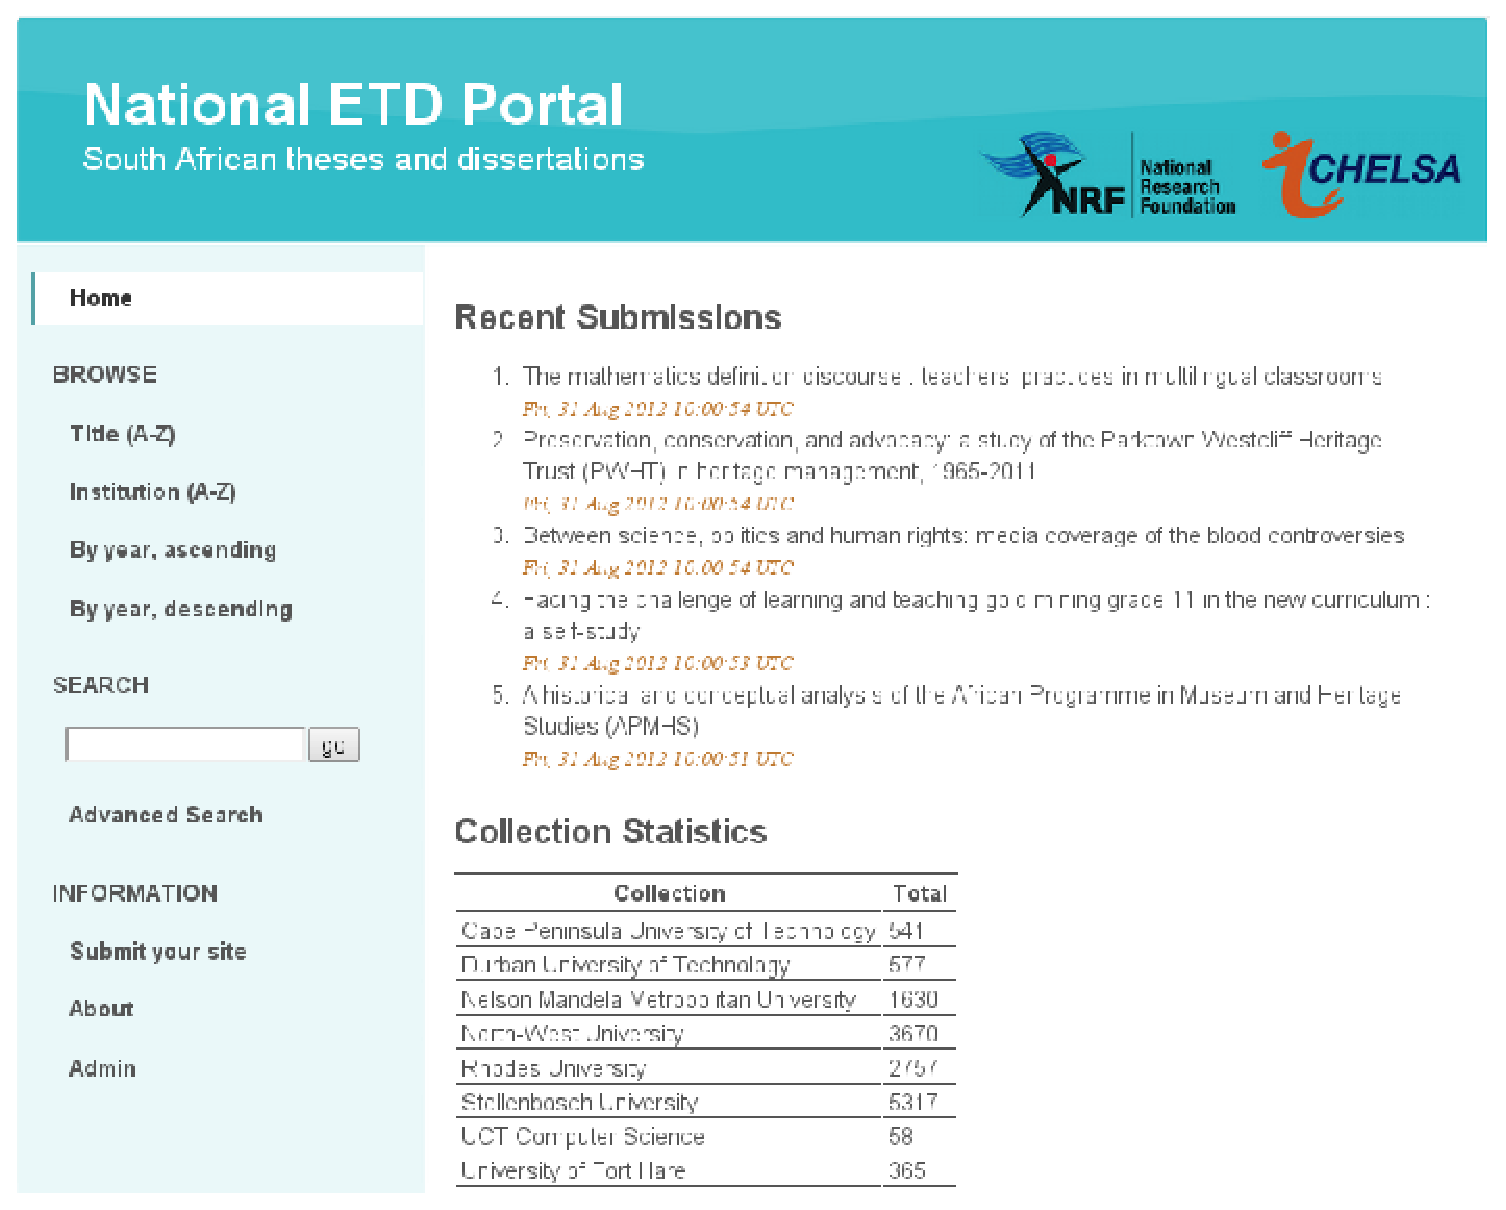
\includegraphics[width=0.95\textwidth]{chapter02/figures/sa-netd-portal.eps}
  }%
  \caption[Screenshot showing the South African NETD portal]{Screenshot showing the South African National Electronic Thesis and Dissertation portal}
  \label{fig:background:digital-libraries:sa-netd-portal}
 %\end{center}

\end{figure}

In addition, a number of federated services are increasingly being implemented
with the aim of making information from heterogeneous services available in
centralised location. Figure~\ref{fig:background:digital-libraries:sa-netd-portal} shows a snapshot of the
South African National Electronic Thesis and Dissertation (NETD) portal\index{NETD}---a federated
service that makes it possible for \glspl{etd}\index{ETD} from various South African universities
to be discovered from a central location.

\begin{figure}
 %\begin{center}
 \centering
  \framebox{%
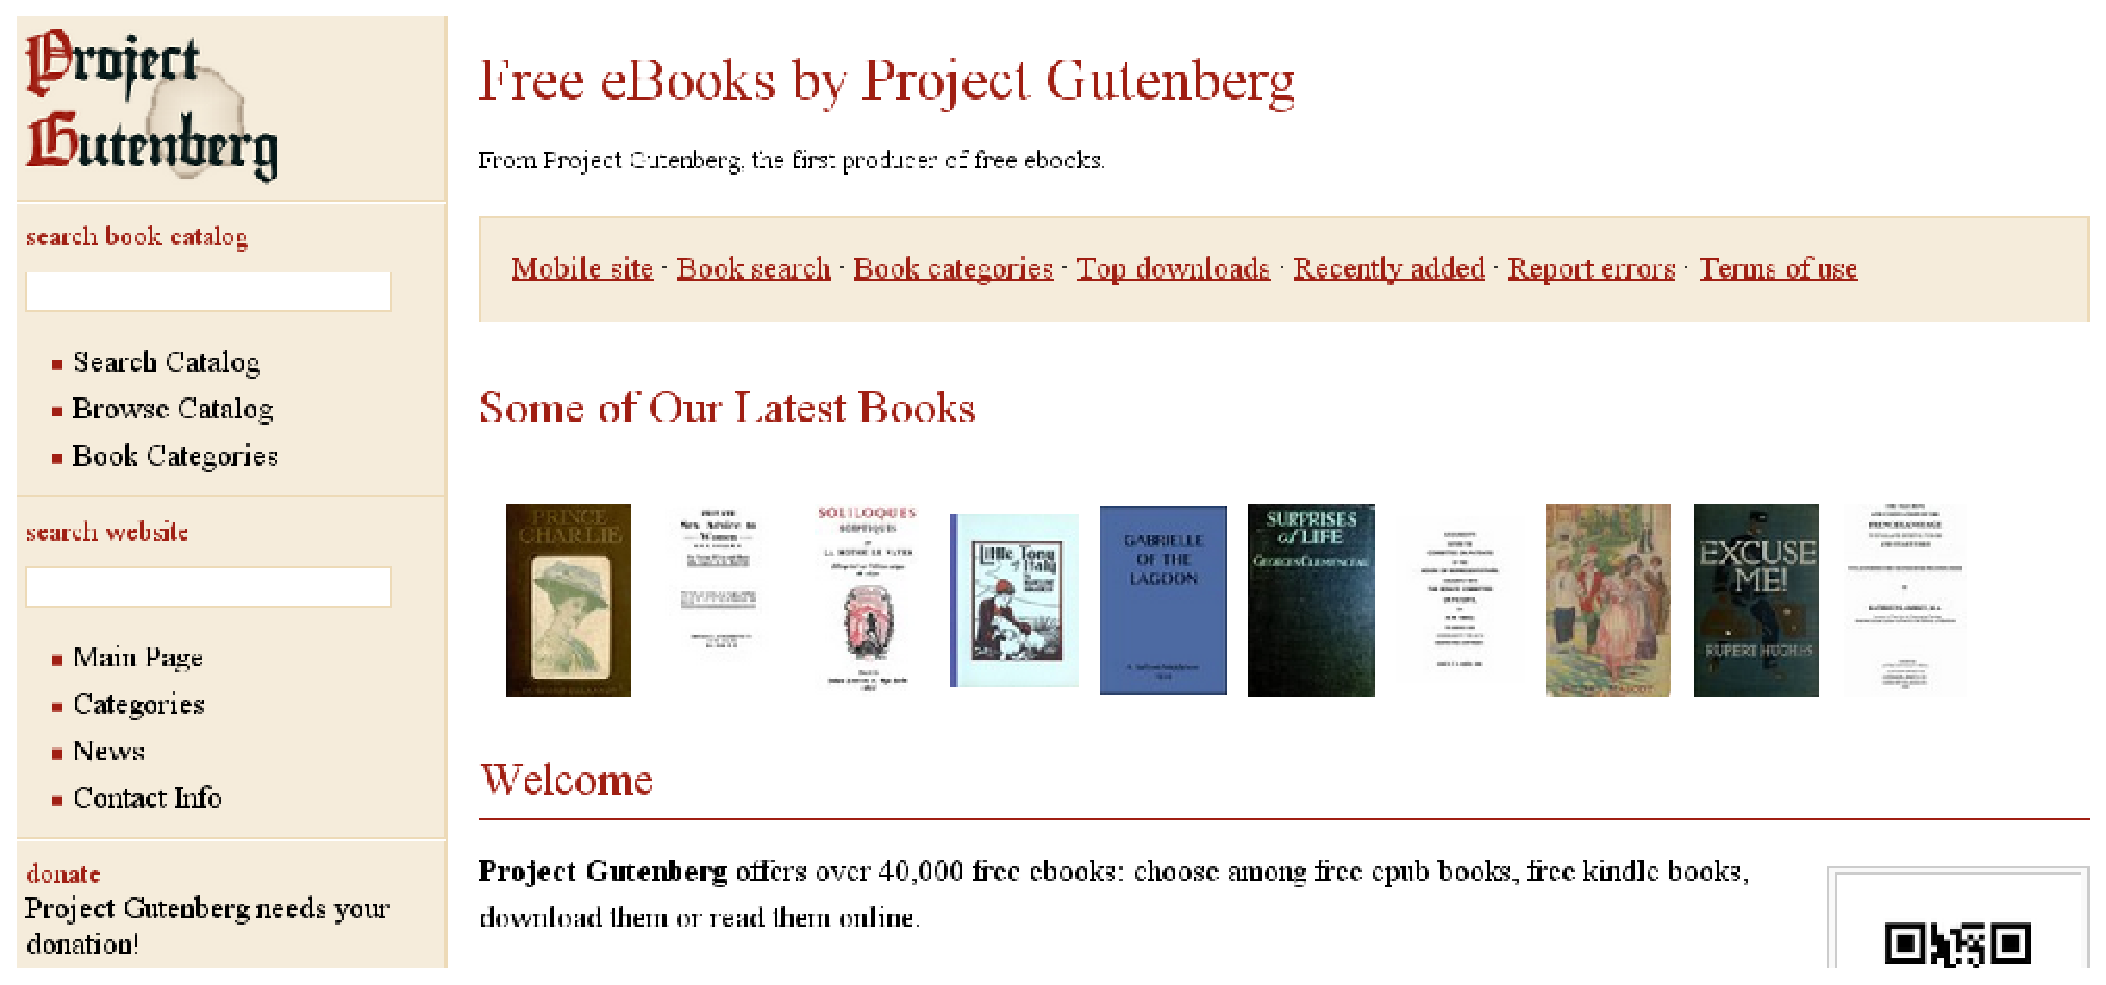
\includegraphics[width=0.95\textwidth]{chapter02/figures/project-gutenberg.eps}
  }%
  \caption{Screenshot showing the Project Gutenburg free ebooks portal}
  \label{fig:background:digital-libraries:project-gutenburg}
 %\end{center}
\end{figure}

\subsection{Summary}
\label{sec:background:digital-libraries:summary}

The massive number of physical copies being digitised, coupled with the increase in the generation of born-digital objects, has created a need for tools and services---\glspl{dl}---for making these objects easily accessible and preservable over long periods of time. The importance of these systems is manifested through their ubiquitous use in varying application domains.

This section broadly defined and described \glspl{dl}, and subsequently discussed some prominent application domains within which are currently used.
\section{Fundamental concepts}\index{Digital Libraries!Concepts}
\label{sec:background:fundamental-concepts}

\subsection{Identifiers}\index{Digital Libraries!Naming Schemes}
\label{sec:background:fundamental-concepts:identifiers}

An identifier is a name given to an entity for current and future reference. Arms \citep{Arms1995} classifies identifiers as vital building blocks for \gls{dl} \index{Digital Libraries} and emphasises their role in ensuring that individual digital objects are easily identified and changes related to the objects are linked to the appropriate objects. He also notes that they are also essential for information retrieval and for providing links between objects.

The importance of identifiers is made evident by the widespread adoption of standardised naming schemes such as \glspl{doi}\footnote{\url{http://www.doi.org}} \citep{Paskin2005,Paskin2010} \index{Digital Libraries!Naming Schemes!DOI}, Handles System\footnote{\url{http://www.handle.net}} and \glspl{purl}\footnote{\url{http://purl.oclc.org}}\index{Digital Libraries!Naming Schemes!PURL}.

\glspl{uri} \citep{RFC39862005} are considered a suitable naming scheme for digital objects primarily because they can potentially be resolved through standard Web protocols; that facilitates interoperability, a feature that is significant in \gls{dl} \index{Digital Libraries} whose overall goal is the widespread dissemination of information.

\subsection{Interoperability}\index{Digital Libraries!Interoperability}
\label{sec:background:fundamental-concepts:interoperability}

Interoperability\index{Interoperability} is a system attribute that enables a system to communicate and exchange information with other heterogeneous systems in a seamless manner. Interoperability\index{Interoperability} makes it possible for services, components and systems developed independently to potentially rely on one another to accomplish certain tasks with the overall goal of having individual components evolve independently, but be able to call on each other, thus exchanging information, efficiently and conveniently \citep{Paepcke1998}⁠. \gls{dl} interoperability has particularly made it possible for federated services \citep{Goncalves2001} to be developed, mainly due to the widespread use of the \gls{oaipmh}.

There are various protocols that have been developed to facilitate interoperability among heterogeneous \glspl{dls}. Prominent interoperability protocols include: Z39.50\index{Z39.50} \citep{Lynch1994}⁠ a client-server protocol used for remote searching; \gls{oaipmh}\index{OAI-PMH} \citep{Lagoze2002}⁠, which has been extensively used for metadata\index{Metadata} harvesting; and RSS\index{RSS} \citep{Winer2007}⁠, a Web based feed format commonly used for obtaining updates on Web resources.

\gls{xml} \index{XML} has emerged as the underlying language used to support a number of these interoperability protocols, largely due to its simplicity and platform independence.

\subsection{Metadata}\index{Digital Libraries!Metadata}
\label{sec:background:fundamental-concepts:metadata}

Metadata\index{Metadata} is representational information that includes pertinent descriptive annotations necessary to understand a resource. Arms \citep{Arms1997}⁠ describes different categories of information as being organised as sets of digital objects---a fundamental unit of the \gls{dl} architecture---that are composed of digital material and key-metadata. He defines the key-metadata as information needed to manage the digital object in a networked environment. The role performed by metadata\index{Metadata} is both implicit and explicit and its functions can be more broadly divided into distinct categories. A typical digital object normally has administrative metadata\index{Metadata} for managing the digital object, descriptive metadata\index{Metadata} to facilitate the discovery of information, structural metadata\index{Metadata} for describing relationships within  the digital object and preservation metadata\index{Metadata} that stores provenance information. Metadata\index{Metadata} is made up of elements that are grouped into a standard set, to achieve a specific purpose, resulting in a metadata\index{Metadata} schema. There are a number of metadata\index{Metadata} schemes that have been developed as standards across various disciplines and they include, among others, Dublin Core\index{Metadata!Schemes!Dublin Core} \citep{DCMI1999}⁠, Learning Object Metadata\index{Metadata} (LOM)\index{Metadata!Schemes!LOM} \citep{IEEE2002}, Metadata\index{Metadata} Encoding and Transmission Standard (METS)\footnote{\url{http://www.loc.gov/standards/mets}}\index{Metadata!Schemes!METS} and Metadata\index{Metadata} Object Description Schema (MODS)\footnote{\url{http://www.loc.gov/standards/mods}}\index{Metadata!Schemes!MODS}⁠. Metadata\index{Metadata} can either be embedded within the digital object---as is the case with Portable Document Format (PDF)\index{PDF} and Hypertext Transfer Markup Language (HTML)\index{HTML} documents---or stored separately with links to the resources being described. Metadata\index{Metadata} in \gls{dl} \index{Digital Libraries} is often stored in databases for easy management and access.

\subsection{Standards}\index{Digital Libraries!Concepts!Standards}
\label{sec:background:fundamental-concepts:standards}

The fast pace at which technology is moving has spawned different types of application software tools. This means that the choice of which technology to use in any given instance differs, thus complicating the process of integrating application software with other heterogeneous software tools. Standards become particularly useful in such situations because they form the basis for developing interoperable tools and services. A standard is a specification---a formal statement of a data format or protocol---that is maintained and endorsed by a recognised standards body \citep[see][chap. 2]{Suleman2010}⁠.

Adopting and adhering to standards has many other added benefits---and Strand et al. \citep{Strand1994} observe that applications that are built on standards are more readily scalable, interoperable and portable, constituting software quality attributes that are important for the design, implementation and maintenance of \glspl{dl}. Standards also play a vital role in facilitating long term preservation of digital objects by ensuring that documents still become easily accessible in the future. This is done by ensuring that the standard itself does not change and by making the standard backwards compatible. Notable use of standards in \gls{dl} \index{Digital Libraries} include the use of \gls{xml}\index{XML} as the underlying format for metadata\index{Metadata} and \gls{oaipmh}\index{OAI-PMH} as an interoperability protocol. Digital content is also stored in well known standards, as is the case with documents that are normally stored in \gls{pdfa}\index{OAI-PMH} format. The use of standards in \glspl{dls}, however, has its own shortcomings; in certain instances, the use of standards can be a very expensive venture as it may involve a lot of cross-domain effort \citep{Lorist2001}⁠.

\subsection{Summary}
\label{sec:background:fundamental-concepts:summary}

A \gls{dls} operates as a specialised type of information system and exhibits certain characteristics to attain its objects. This section discussed fundamental concepts, associated to \glspl{dls}, that help form the necessary building blocks for implementing \glspl{dl}.
\section[Frameworks]{Digital Libraries frameworks}\index{Digital Libraries!Frameworks}
\label{sec:background:reference-models-frameworks}

A reference model is an abstract framework that provides basic concepts used to understand the relationships among items in an environment. The \gls{oasis} \citep{MacKenzie2006}⁠ states that a reference model consists of a minimal set of unifying concepts, axioms and relationships within a particular problem domain, and is independent of specific standards, technologies, implementations or other concrete details.

Several \gls{dl} frameworks \citep{Gonccalves2004,Kahn2006} and reference models \citep{Candela2007a} have addressed specific problems in \gls{dls} architectural design and implementation. A discussion of some prominent reference models now follows.

%\subsection{Warwick Framework}
%\label{sec:background:reference-models-frameworks:warwick}
%
%Xxx xxx
%
%Xxx xxx
% @comment: Clearly, this right here is not in anyway relevant.
%
\subsection[5S framework]{Streams, Structures, Spaces and Societies}
\label{sec:background:reference-models-frameworks:5s}

The \gls{5s} framework\index{Digital Libraries!Frameworks!5S} is a unified formal theory for \glspl{dl}. It is an attempt to define and easily understand the complex nature of \glspl{dl} in a rigorous manner. The framework is based on formal definitions, and abstraction of five fundamental concepts---Streams, Structures, Spaces, Scenarios and Societies \citep{Gonccalves2004}⁠.  The five concepts, together with their corresponding definitions and examples, are summarised in Table~\ref{tab:background:reference-models-frameworks:5s}.

\tablespacing
%%%%%\begin{longtable}{p{0.15\linewidth} p{0.40\linewidth} p{0.30\linewidth}}
\begin{longtable}{
>{\arraybackslash}p{0.15\linewidth}|
>{\arraybackslash}p{0.40\linewidth}|
>{\arraybackslash}p{0.30\linewidth}}

\caption{Summary of key aspects of the 5S framework}
\label{tab:background:reference-models-frameworks:5s} \\
 %%%%%\toprule
 %%%%%\hline
 \textbf{Concept} & \textbf{Description} & \textbf{Examples} \\
 %%%%%\midrule
 \cline{1-3}
 \endfirsthead
 
 \caption[]{(continued)}\\
 %%%%%\toprule
 %%%%%\hline
 \textbf{Concept} & \textbf{Description} & \textbf{Examples} \\
 %%%%%\midrule
 \cline{1-3}
 \endhead
 
 % Page footer
 %%%%%\midrule
 %%%%%\hline
 \multicolumn{3}{r}{(Continued on next page)} \\
 \endfoot
 
 % Last page footer
 %%%%%\bottomrule
 \endlastfoot
 
 \textbf{Streams} &
 {Streams represent a sequence of elements of an arbitrary type} &
 {Text, video, audio, software} \\
 
 \cline{1-3}
 %\cmidrule[0.1pt](l{0.5em}r{0.5em}){1-3}
 
 \textbf{Structures} &
 {Structures specify the organisation of different parts of a whole} &
 {Collection, document, metadata} \\
 
 \cline{1-3}
 %\cmidrule[0.1pt](l{0.5em}r{0.5em}){1-3}
 
 \textbf{Spaces} &
 {Spaces are sets of objects, with associated operations, that obey certain constants} &
 {User interface, index} \\
 
 \cline{1-3}
 %\cmidrule[0.1pt](l{0.5em}r{0.5em}){1-3}
 
 \textbf{Scenarios} &
 {Scenarios define details for the behaviour of services} &
 {Service, event, action} \\
 
 \cline{1-3}
 %\cmidrule[0.1pt](l{0.5em}r{0.5em}){1-3}
 
 \textbf{Societies} &
 {Societies represent sets of entities and the relationships among them} &
 {Community, actors, relationships, attributes, operations} \\
 
\end{longtable}

\bodyspacing

In the context of the aims of \glspl{dl}, Gon\c{c}alves et al. \citep{Gonccalves2004} outline an association between \gls{5s} and some aims of a \gls{dls}, with Streams being aligned with the overall communication and consumption of information by end users; Structures supporting the organisation of information; Spaces dealing with the presentation and access to information in usable and effective ways; Scenarios providing the necessary support for defining and designing services; and Societies defining how a \gls{dl} satisfies the overall information needs of end users.

However, Candela et al. \citep{Candela2007}⁠ state that the \gls{5s} framework is very general-purpose and thus less immediate. The \gls{5s} framework is also arguably aimed at formalising the \gls{dl} aspects, as opposed to prescribing specific design guidelines.

\subsection[Kahn\& Wilensky framework]{Kahn and Wilensky framework}
\label{sec:background:reference-models-frameworks:kahn-wilensky}

This is a generic information system framework for distributed digital object services with digital objects as the main building blocks. The framework is based on an open architecture that supports large and distributed digital information services. Kahn and Wilensky\index{Digital Libraries!Frameworks!Kahn/Wilensky} \citep{Kahn2006}⁠ describe the framework in terms of the fundamental aspects of an open and distributed infrastructure, and how the basic components in such an infrastructure support storage, accessibility and management of digital objects.

In addition to a high level conceptual description of such a distributed information system, the framework primarily focuses on the network-based aspects of such an infrastructure \citep{Kahn2006}. Specifically, an elaborate description of how digital objects should be accessed via a \gls{rap} is outlined. The framework also proposes the use of a handle server infrastructure as a means for mapping registered digital objects.

In essence, the framework merely prescribes conventional methods for the unique identification, reliable location, and flexible access to digital objects.

\subsection{DELOS reference model}
\label{sec:background:reference-models-frameworks:delos}

The DELOS\index{Digital Libraries!Frameworks!DELOS} Network of Excellence on \glspl{dl}\footnote{\url{http://www.delos.info}} was a European Union co-funded project aimed at integrating and coordinating research activities in \glspl{dl}. The DELOS working group published a manifesto that establishes principles that facilitate the capture of the full spectrum of concepts that play a role in \glspl{dl} \citep{Candela2007a}⁠. The result of this project was a reference model---the DELOS \gls{dl} reference model---comprising to a set of concepts and relationships that collectively attempt to capture various entities of the \gls{dl} universe.

A fundamental part of the DELOS reference model is the \gls{dl} Manifesto, that presents a \gls{dl} as a three-tier framework consisting of a \gls{dl}, representing an organisation; a \gls{dls}, for implementing \gls{dl} services; and a \gls{dlms}, comprising of tools for administering the \gls{dls}. Figure~\ref{fig:background:reference-models-frameworks:delos}\footnote{Permission to reproduce this image was granted by Donatella Castelli} shows the interaction among the three sub-systems.

The reference model further identifies six core concepts that provide a firm foundation for \glspl{dl}. These six concepts---Content, User, Functionality, Quality, Policy and Architecture---are enshrined within the \gls{dl} and the \gls{dls}. All concepts, with the exceptions of the Architecture concept, appear in the definition of the \gls{dl}. The Architecture is, however, handled by the \gls{dls} definition \citep{Candela2007}⁠.

The Architecture component, addressed by the \gls{dls}, is particularly important in the context of this research as it represents the mapping of the functionality and content on to the hardware and software components. Candela et al. \citep{Candela2007}⁠ attribute the inherent complexity of \glspl{dl} and the interoperability challenges across \glspl{dl} as the two primary reasons for having Architecture as a core component.

Another important aspect of the reference model, directly related to this research, are the reference frameworks needed to clarify the \gls{dl} universe at different levels of abstraction. The three reference development frameworks are: Reference Model, Reference Architecture, and Concrete Architecture. In the context of architectural design, the Reference Architecture is vital as it provides a starting point for the development of an architectural design pattern, thus paving the way for an abstract solution.

\begin{figure}
 %\begin{center}
  \centering
  \framebox[\textwidth]{%
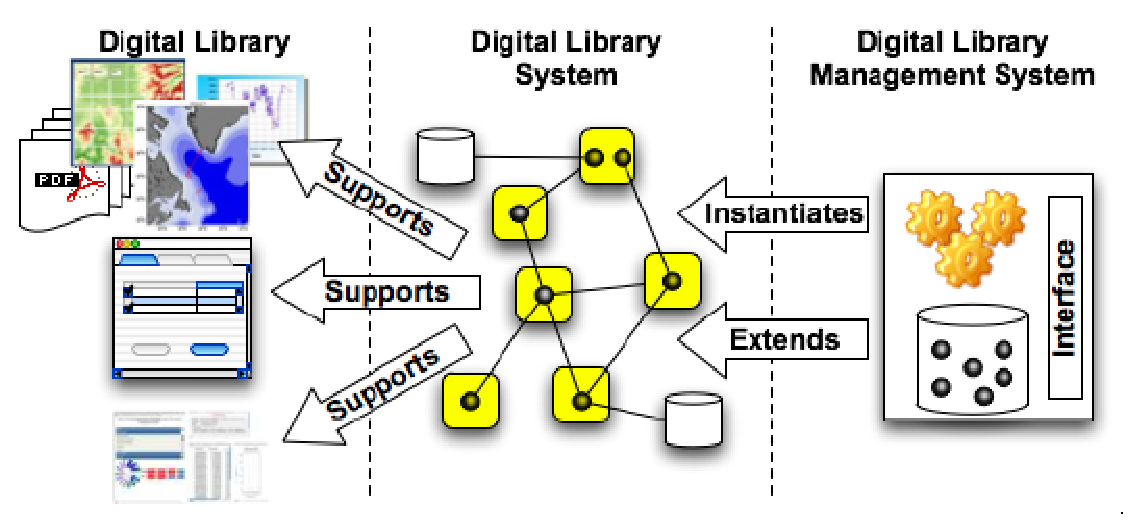
\includegraphics[width=0.95\textwidth]{%
chapter02/figures/delos-dl-dls-dlms.eps}%
}%
\caption[DL, DLS and DLMS: A three-tier framework]{DL, DLS and DLMS: A three-tier framework}
\label{fig:background:reference-models-frameworks:delos}
% \end{center}
\end{figure}

\subsection{Summary}
\label{sec:background:reference-models-frameworks:summary}

The motivation behind building both the reference models was largely influenced by the need to understand the complexity inherent in \glspl{dl}. The idea of designing a \gls{dl} architecture based on direct user needs is not taken into account in existing reference models, although the DELOS Reference Architecture does have a provision for the development of specific architectural design patterns. The DELOS Reference Architecture is in actual fact considered to be mandatory for the development of good quality \glspl{dls}, and for the integration and reuse of the system components.
\section[Software platforms]{Software platforms}\index{Digital Libraries!Software}
\label{sec:background:digital-libraries-software}

There are a number of different \gls{dl} software tools currently available. The ubiquitous availability of these tools could, in part, be as a result of specialised problems that these solutions are designed to solve. This section discusses seven prominent \gls{dl} software platforms.

\subsection{CDS Invenio}

CDS Invenio\index{Digital Libraries!Software!CDS Invenio}, formally known as CDSware\index{CDSware}, is an open source repository software, developed at CERN\footnote{\url{http://www.cern.ch}} and originally designed to run the CERN document server\footnote{\url{http://cdsweb.cern.ch}}. CDS Invenio provides an application framework with necessary tools and services for building and managing a \gls{dl} \citep{Vesely2004}.

The ingested digital objects' metadata\index{Metadata} records are internally converted into a MARC\index{MARC} 21 ---MARCXML--- representation structure, while the actually fulltext bitstreams are automatically converted into PDF\index{PDF}. This ingested content is subsequently accessed by downstream services via OAI service providers, email alerts and search engines \citep{Pepe2005}.

The implementation is based on a modular architecture. It is implemented using the Python Programming language, runs within an Apache/Python\index{Python} Web application server, and makes use of a MySQL\index{MySQL} backend database server for storage of metadata\index{Metadata} records.

\subsection{DSpace}

DSpace\index{Digital Libraries!Software!DSpace} is an open-source repository software that was specifically designed for storage of digital research and institutional materials. The architectural design was largely influenced by the need for materials to be stored and accessed over long periods of time \citep{Transley2003}.

The digital object metadata\index{Metadata} records are encoded using qualified Dublin Core\index{Dublin Core}---to facilitate effective resource description. Digital objects are accessed and managed via application layer services that support protocols such as OAI-PMH\index{OAI-PMH}.

DSpace\index{DSpace} is organised into a three-tier architecture, composed of: an application layer; a business logic layer; and a storage layer. The storage layer stores digital content within an asset store---a designated area within the operating system's filesystem; or can alternatively use a storage resource broker. The digital objects ---bitstreams\index{Bitstream} and corresponding metadata records--- are stored within a relational database management system \citep{Smith2003,Tansley2003a}. Furthermore software is implemented using the Java programming languages, and is thus deployed within a Servlet\index{Servlet} Engine. However, this architectural design approach arguably makes it difficult to recover digital objects in the event of a disaster since technical expertise would be required.

\subsection{EPrints}

EPrints\index{Digital Libraries!Software!EPrints} is an archival software that designed to create highly configurable Web-based archives. The initial design of the software can be traced back to a time when there was a need to foster open access to research publications, and provides a flexible \gls{dl} platform for building repositories \citep{Gutteridge2002}.

Eprints\index{EPrints} records are represented as data objects that contain metadata\index{Metadata}. The software's plugin architecture enables the flexible design and development of export plugins capable of converting repository objects into a variety of other formats. This technique effectively makes it possible for the data objects to be disseminated via different services---such as OAI data provider modules.

EPrints\index{EPrints} is implemented using Perl\index{Perl}, runs within an Apache HTTP\index{HTTP} server and uses a MySQL\index{MySQL} database server backend to store metadata records. However, the actual files in the archive are stored on the filesystem.

\subsection{ETD-db}

The ETD-db\index{Digital Libraries!Software!ETD-db} digital repository software for depositing, accessing and managing \gls{etd} collections. The software is more oriented towards helping facilitate the access and management of \glspl{etd}.

The software was initially developed as is a series of Web pages and additional Perl\index{Perl} scripts that interact with a MySQL\index{MySQL} database backend \citep{ETDdbHome}. However, the latest version---\gls{etd} 2.0---is a Web application, implemented using the Ruby on Rails Web application framework. This was done in an effort to handle \gls{etd} collections more reliably and securely. In addition, the latest version is able to work with any relational database and can be hosted on any Web server that supports Ruby on Rails \citep{Park2011}.

\subsection{Fedora Commons}

Fedora\index{Digital Libraries!Software!Fedora-Commons} is an open source digital content repository framework designed for managing and delivering complex digital objects \citep{Lagoze2006}.

The Fedora architecture is based on the Kahn and Wilensky framework \citep{Kahn2006}, discussed in Section~\ref{sec:background:reference-models-frameworks:kahn-wilensky}, with a distributed model that makes it possible for complex digital objects to make reference to content stored on remote storage systems. 

The Fedora framework is composed of loosely coupled services ---implemented using the Java programming language--- that interact with each other to provide the functionally of the Web service as a whole. The Web service functionalities are subsequently exposed via REST\index{REST} and SOAP\index{SOAP} interfaces.

\subsection{Greenstone}

Greenstone\index{Digital Libraries!Software!Greenstone} is an open source digital collection building and distributing software. The software's ability to redistribute digital collections on self-installing CD-ROMs has made it a popular tool of choice in regions with very limited bandwidth \citep{Witten2001}.

The most recent version---Greenstone3 \citep{Greenstone3}---is implemented in Java\index{Java}, making it platform independent. It was redesigned to improve the dynamic nature of the Greenstone toolkit and to further lower the potential overhead incurred by collection developers. In addition, it is distributed and can thus be spread across different servers. Furthermore, the new architecture is modular, utilising independent agent modules that communicate using single message calls \citep{Bainbridge2004}.

Greenstone uses \gls{xml}\index{XML} to encode resource metadata records ---XLinks\index{XLink} are used to represent relationships between other documents. Using this strategy, resources and documents are retrievable through \gls{xml}\index{XML} communication. Furthermore, indexing documents enables effective searching and browsing of resources. 

The software operates within an Apache Tomcat Servlet Engine.

\subsection{Omeka}

Omeka\index{Digital Libraries!Software!Omeka} is a Web-based publishing platform for publishing digital archives and collections \citep{Kucsma2010}. It is standards-based and highly interoperable---it makes use of unqualified Dublin Core and is \gls{oaipmh} compliant. In addition, it is relatively easy to use and has a very flexible design, which is customisable and highly extensible via the use of plugins.

Omeka is implemented using the PHP\index{PHP} scripting language and uses MySQL\index{MySQL} database as a backend for storage of metadata\index{Metadata} records. However, the ingested resources---bitstreams--- are stored on the filesystem.

\subsection{Summary}

Table~\ref{tab:background:related-work:digital-libraries-software:floss-matrix} is a feature matrix of the digital libraries software discussed in this section.

\tablespacing
%%%\begin{longtable}{p{0.03\linewidth} p{0.30\linewidth} p{0.03\linewidth}
%%%p{0.03\linewidth} p{0.03\linewidth} p{0.03\linewidth} p{0.03\linewidth}
%%%p{0.03\linewidth} p{0.03\linewidth}}
\begin{longtable}{
>{\centering\arraybackslash}p{0.008\linewidth}|
>{\arraybackslash}p{0.55\linewidth}|
>{\centering\arraybackslash}p{0.005\linewidth}|
>{\centering\arraybackslash}p{0.005\linewidth}|
>{\centering\arraybackslash}p{0.005\linewidth}|
>{\centering\arraybackslash}p{0.005\linewidth}|
>{\centering\arraybackslash}p{0.005\linewidth}|
>{\centering\arraybackslash}p{0.005\linewidth}|
>{\centering\arraybackslash}p{0.005\linewidth}
}
 
\caption{Feature matrix for some popular DL FLOSS software tools}
\label{tab:background:related-work:digital-libraries-software:floss-matrix} \\
 %%%%%\toprule
 %%%%%\cline{3-9}
 \multicolumn{1}{c}{} & 
 \multicolumn{1}{c|}{} & 
 \multicolumn{1}{c|}{\begin{sideways}\textbf{CDS Invenio}\end{sideways}} &
 \multicolumn{1}{c|}{\begin{sideways}\textbf{DSpace}\end{sideways}} &
 \multicolumn{1}{c|}{\begin{sideways}\textbf{EPrints}\end{sideways}} &
 \multicolumn{1}{c|}{\begin{sideways}\textbf{ETD-db}\end{sideways}} &
 \multicolumn{1}{c|}{\begin{sideways}\textbf{Fedora Commons}\end{sideways}} &
 \multicolumn{1}{c|}{\begin{sideways}\textbf{Greenstone}\end{sideways}} &
 \multicolumn{1}{c}{\begin{sideways}\textbf{Omeka}\end{sideways}} \\
 %%%%%\midrule
 \cline{1-9}
 \endfirsthead
 
 \caption[]{(continued)}\\
 %%%%%\toprule
 %%%%%\cline{3-9}
 \multicolumn{1}{c}{} & 
 \multicolumn{1}{c|}{} & 
 \multicolumn{1}{c|}{\begin{sideways}\textbf{CDS Invenio}\end{sideways}} &
 \multicolumn{1}{c|}{\begin{sideways}\textbf{DSpace}\end{sideways}} &
 \multicolumn{1}{c|}{\begin{sideways}\textbf{EPrints}\end{sideways}} &
 \multicolumn{1}{c|}{\begin{sideways}\textbf{ETD-db}\end{sideways}} &
 \multicolumn{1}{c|}{\begin{sideways}\textbf{Fedora Commons}\end{sideways}} &
 \multicolumn{1}{c|}{\begin{sideways}\textbf{Greenstone}\end{sideways}} &
 \multicolumn{1}{c}{\begin{sideways}\textbf{Omeka}\end{sideways}} \\
 \cline{1-9}
 \endhead
 
 % Page footer
 %%%%%\midrule
 \cline{1-9}
 \multicolumn{9}{c}{(Continued on next page)} \\
 \endfoot
 
 % Last page footer
 %%%%%\bottomrule
 \endlastfoot
 
 \multirow{6}{*}{\begin{sideways}\textbf{Storage} \end{sideways}} &
 \textbf{Complex object support}&
 {}&
 {}&
 {}&
 {}&
 {X}&
 {}&
 {}\\
 
 %%%%%\cmidrule[0.1pt](l{0.5em}r{0.5em}){2-9}
 \cline{3-9}
 
 &
 \textbf{Dublin Core support for metadata} &
 {}&
 {X}&
 {X}&
 {}&
 {X}&
 {X}&
 {X}\\
 
 %%%%%\cmidrule[0.1pt](l{0.5em}r{0.5em}){2-9}
 \cline{3-9}
  
 &
 \textbf{Metadata is stored in database} &
 {X}&
 {X}&
 {X}&
 {X}&
 {X}&
 {X}&
 {X}\\
 
 %%%%%\cmidrule[0.1pt](l{0.5em}r{0.5em}){2-9}
 \cline{3-9}
 
 {} &
 %%%%%\begin{sideways}\textbf{} \end{sideways} &
 \textbf{Metadata can be stored on filesystem} &
 {}&
 {}&
 {}&
 {}&
 {}&
 {X}&
 {}\\
 
 %%%%%\cmidrule[0.1pt](l{0.5em}r{0.5em}){2-9}
 \cline{3-9}
 
  &
 \textbf{Supports distributed repositories} &
 {X}&
 {X}&
 {X}&
 {X}&
 {X}&
 {X}&
 {X}\\
 
 %%%%%\cmidrule[0.1pt](l{0.5em}r{0.5em}){2-9}
 \cline{1-9}
 
  &
 \textbf{Object relationship support} &
 {}&
 {}&
 {}&
 {}&
 {X}&
 {}&
 {X}\\
 
 %%%%%\cmidrule[0.1pt](l{0.5em}r{0.5em}){1-9}
 \cline{3-9}
 
 \multirow{5}{*}{\begin{sideways}\textbf{Services} \end{sideways}} &
 \textbf{Extensible via plugins} &
 {X}&
 {X}&
 {X}&
 {}&
 {X}&
 {X}&
 {X}\\
 
 %%%%%\cmidrule[0.1pt](l{0.5em}r{0.5em}){2-9}
 \cline{3-9}
 
  &
 \textbf{OAI-PMH complaint} &
 {X}&
 {X}&
 {X}&
 {X}&
 {X}&
 {X}&
 {X}\\
 
 %%%%%\cmidrule[0.1pt](l{0.5em}r{0.5em}){2-9}
 \cline{3-9}
  
 %\begin{sideways}\textbf{Technologies}\end{sideways} &
 \begin{sideways}\textbf{}\end{sideways} &
 \textbf{Platform independent} &
 {}&
 {X}&
 {X}&
 {}&
 {X}&
 {X}&
 {X}\\
 
 %%%%%\cmidrule[0.1pt](l{0.5em}r{0.5em}){2-9}
 \cline{3-9}
  
  &
 \textbf{Supports Web services} &
 {}&
 {X}&
 {}&
 {}&
 {X}&
 {X}&
 {}\\
 
 %%%%%\cmidrule[0.1pt](l{0.5em}r{0.5em}){2-9}
 \cline{3-9}
  
  &
 \textbf{URI support(e.g. DOIs)} &
 {}&
 {X}&
 {}&
 {}&
 {X}&
 {}&
 {}\\
 
 %%%%%\cmidrule[0.1pt](l{0.5em}r{0.5em}){2-9}%
 \cline{1-9}
 
 \multirow{7}{*}{\begin{sideways}\textbf{Features} \end{sideways}} &
 \textbf{Alternate accessibility (e.g. CD-ROM)} &
 {}&
 {}&
 {}&
 {}&
 {}&
 {X}&
 {}\\
 
 %%%%%\cmidrule[0.1pt](l{0.5em}r{0.5em}){2-9}
 \cline{3-9}

   &
 \textbf{Easy to setup, configure and use} &
 {}&
 {}&
 {X}&
 {}&
 {}&
 {X}&
 {X}\\
 
 %%%%%\cmidrule[0.1pt](l{0.5em}r{0.5em}){2-9}
 \cline{3-9}
 
   &
 \textbf{Handles different file formats} &
 {X}&
 {X}&
 {X}&
 {}&
 {X}&
 {X}&
 {X}\\
 
 %%%%%\cmidrule[0.1pt](l{0.5em}r{0.5em}){1-9}
 \cline{3-9}
 
  &
 \textbf{Hierarchical collection structure} &
 {}&
 {X}&
 {X}&
 {}&
 {X}&
 {X}&
 {}\\
 
 %%%%%\cmidrule[0.1pt](l{0.5em}r{0.5em}){2-9}
 \cline{3-9}
 
 %\begin{sideways}\textbf{Features}\end{sideways} &
 \begin{sideways}\textbf{}\end{sideways} &
 \textbf{Horizontal market software} &
 {X}&
 {X}&
 {X}&
 {}&
 {X}&
 {X}&
 {X}\\

 %%%%%\cmidrule[0.1pt](l{0.5em}r{0.5em}){2-9}
 \cline{3-9}
 
   &
 \textbf{Web interface} &
 {X}&
 {X}&
 {X}&
 {X}&
 {X}&
 {X}&
 {X}\\
 
 %%%%%\cmidrule[0.1pt](l{0.5em}r{0.5em}){2-9}
 \cline{3-9}
 
   &
 \textbf{Workflow support} &
 {X}&
 {X}&
 {X}&
 {X}&
 {}&
 {}&
 {}\\
 
\end{longtable}

\bodyspacing
\section{Minimalist philosophy}\index{Minimalism}
\label{sec:background:simple-architectures}

The application of minimalism\index{Minimalism} in both software and hardware designs is widespread, and has been employed since the early stages of computing. The Unix\index{Unix} operating system is perhaps one prominent example that provides a unique case of the use of minimalism as a core design philosophy, and Raymond \citep{Raymond2004} outlines the benefits, on the Unix platform, of designing for simplicity\index{Simplicity}. This section discusses relevant architectures that were designed with simplicity\index{Simplicity} in mind.

% Not quite sure if this subsubsection is relevant---might have to figure out
% how to incorporate this information in a different section
%\subsection{Ubiquitous Access to Information}
%\label{sec:background:related-work:ubiquitous-access}
%Various solutions have been devised to facilitate ubiquitous access to
%knowledge by overcoming problems experienced in resource constrained
%environments.

%\subsubsection{One Laptop Per Child Project}
%\label{sec:background:related-work:ubiquitous-access}

%xxxx xxxx

%\subsection{World Wide Web}
%\label{sec:background:world-wide-web}
% NOT YET SURE ABOUT INCLUDING THE WEB HERE
%xxx xxx

\subsection[Dublin Core]{Dublin Core element set}
\label{sec:background:simple-architectures:dublin-core-element-set}

The Dublin Core\index{Dublin Core} metadata\index{Metadata} element set defines a set of 15 resource description properties that are potentially applicable to a wide range of resources. One of the main goals of the Dublin Core\index{Dublin Core} element set is aimed at keeping the element set as small and simple as possible to facilitate the creation of resource metadata by non-experts \citep{Hillmann2005}.

\tablespacing
%%%%%\begin{longtable}{p{0.15\linewidth} p{0.75\linewidth}}
\begin{longtable}{
>{\arraybackslash}p{0.16\linewidth}|
>{\arraybackslash}p{0.74\linewidth}}
 
 \caption{Simple unqualified Dublin Core element set}
\label{tab:background:simple-architectures:dublin-core-element-set} \\
 %%%%%\toprule
 %%%%%\hline
 \textbf{Element} & \textbf{Element Description}\\
 %%%%%\midrule
 \cline{1-2}
 \endfirsthead
 
 \caption[]{(continued)}\\
 %%%%%\toprule
 %%%%%\hline
 \textbf{Element} & \textbf{Element Description}\\
 %%%%%\midrule
 \cline{1-2}
 \endhead
 
 % Page footer
 %%%%%\midrule
 %%%%%\hline
 \multicolumn{2}{r}{(Continued on next page)} \\
 \endfoot
 
 % Last page footer
 %%%%%\bottomrule
 \endlastfoot
 
 \textbf{Contributor} &
 {An entity credited for making the resource available} \\
 
 \cline{1-2}
 %\cmidrule[0.1pt](l{0.5em}r{0.5em}){1-2}
 
 \textbf{Coverage} &
 {Location specific details associated to the resource} \\
 
 \cline{1-2}
 %\cmidrule[0.1pt](l{0.5em}r{0.5em}){1-2}
 
 \textbf{Creator} &
 {An entity responsible for creating the resource} \\
 
 \cline{1-2}
 %\cmidrule[0.1pt](l{0.5em}r{0.5em}){1-2}
 
 \textbf{Date} &
 {A time sequence associated with the resource life-cycle} \\

 \cline{1-2}
 %\cmidrule[0.1pt](l{0.5em}r{0.5em}){1-2}
 
 \textbf{Description} &
 {Additional descriptive information associated to the resource} \\

 \cline{1-2}
 %\cmidrule[0.1pt](l{0.5em}r{0.5em}){1-2}
 
 \textbf{Format} &
 {Format specific attributes associated with the resource} \\

 \cline{1-2}
 %\cmidrule[0.1pt](l{0.5em}r{0.5em}){1-2}
 
 \textbf{Identifier} &
 {A name used to reference the resource} \\

 \cline{1-2}
 %\cmidrule[0.1pt](l{0.5em}r{0.5em}){1-2}
 
 \textbf{Language} &
 {The language used to publish the resource} \\

 \cline{1-2}
 %\cmidrule[0.1pt](l{0.5em}r{0.5em}){1-2}
 
 \textbf{Publisher} &
 {An entity responsible for making the resource available} \\

 \cline{1-2}
 %\cmidrule[0.1pt](l{0.5em}r{0.5em}){1-2}

 \textbf{Relation} &
 {Other resource(s) associated with the resource} \\

 \cline{1-2}
 %\cmidrule[0.1pt](l{0.5em}r{0.5em}){1-2}
 
 \textbf{Rights} &
 {The access rights associated with the resource} \\

 \cline{1-2}
 %\cmidrule[0.1pt](l{0.5em}r{0.5em}){1-2}
 
 \textbf{Source} &
 {The corresponding resource where the resource is derived from} \\

 \cline{1-2}
 %\cmidrule[0.1pt](l{0.5em}r{0.5em}){1-2}
 
 \textbf{Subject} &
 {The topic associated to the resource} \\

 \cline{1-2}
 %\cmidrule[0.1pt](l{0.5em}r{0.5em}){1-2}
 
 \textbf{Title} &
 {The name of the resource} \\

 \cline{1-2}
 %\cmidrule[0.1pt](l{0.5em}r{0.5em}){1-2}
 
 \textbf{Types} &
 {The resource type} \\
 
\end{longtable}

\bodyspacing

The simplicity\index{Simplicity} of the element set arises from the fact that the 15 elements form the smallest possible set of elements required to describe a generic resource. In addition, as shown in Table~\ref{tab:background:simple-architectures:dublin-core-element-set}, the elements are self explanatory, effectively making it possible for a large section of most communities to make full use of the framework. Furthermore, all the elements are repeatable and at the same time optional. This flexibility of the scheme is, in part, the research why it is increasingly becoming popular.

\subsection[Wikis]{Wiki software}\index{Wiki}
\label{sec:background:simple-architectures:wiki-software}

Wiki software allows users to openly collaborate with each other through the process of creation and modification of Web page content \citep{Leuf2001}. The success of Wiki software is, in part, attributed to the growing need for collaborative Web publishing tools. However, the simplicity\index{Simplicity} in the way content is managed, to leverage speed, flexibility and easy of use, is arguably the major contributing factor to their continued success. The strong emphasis on simplicity\index{Simplicity} in the design of Wikis is evident in Cunningham's original description: ``The simplest online database that could possibly work'' \citep{Ward1995,Leuf2001}.

\subsection[XML]{Extensible markup language}
\label{sec:background:simple-architectures:extensible-markup-language}

\gls{xml}\index{XML} is a self-describing markup language that was specifically designed to transport and store data. \gls{xml} provides a hardware- and software-independent mode for carrying information, and was design for ease of use, implementation and interoperability from the onset. This is in fact evident from the original design goals that, in part, emphasised for the language to be easy to create documentations, easy to write programs for processing the documents and straightforwardly usable over the Internet \citep{Bray2008}.

\gls{xml} has become one of the most commonly used tool for transmission of data in various applications due to the following reasons.

\begin{itemize}
 \item Extensibility through the use of custom extensible tags
 \item Interoperability by being usable on a wide variety of hardware and software platforms
 \item Openness through the open and freely available standard
 \item Simplicity of resulting documents, effectively making them readable by machines and humans
\end{itemize}

The simplicity\index{Simplicity} of \gls{xml} particularly makes it an easy and flexible tool to work with, in part, due to the fact that the \gls{xml} document syntax is composed of a fairly minimal set of rules. Furthermore, the basic minimal set of rules can be expanded to grow more complex structures as the need arises.

\subsection[OAI-PMH]{OAI protocol for metadata harvesting}
\label{sec:background:oaipmh-protocol-for-metadata-harvesting}

The \gls{oaipmh} \index{OAI-PMH} is a metadata harvesting interoperability framework \citep{Lagoze2002}. The protocol only defines a set of six request verbs\index{OAI-PMH!Verbs}, shown in Table~\ref{tab:background:simple-architectures:oaipmh-request-verbs}, that data providers need to implement. Downstream service providers then harvest metadata as a basis for providing value-added services.

\tablespacing
%%%%%\begin{longtable}{p{0.30\linewidth} p{0.60\linewidth}}
\begin{longtable}{
>{\arraybackslash}p{0.30\linewidth}|
>{\arraybackslash}p{0.60\linewidth}}
 
 \caption{OAI-PMH request verbs}
\label{tab:background:simple-architectures:oaipmh-request-verbs} \\
 %%%%%\toprule
 %%%%%\hline
 \textbf{Request Verb} & \textbf{Description}\\
 %%%%%\midrule
 \cline{1-2}
 \endfirsthead
 
 \caption[]{(continued)}\\
 %%%%%\toprule
 %%%%%\hline
 \textbf{Request Verb} & \textbf{Description}\\
 %%%%%\midrule
 \cline{1-2}
 \endhead
 
 % Page footer
 %%%%%\midrule
 %%%%%\hline
 \multicolumn{2}{r}{(Continued on next page)} \\
 \endfoot
 
 % Last page footer
 %%%%%\bottomrule
 \endlastfoot

 \textbf{GetRecord} &
 {This verb facilitates retrieval of individual metadata records} \\

 \cline{1-2}
 %\cmidrule[0.1pt](l{0.5em}r{0.5em}){1-2}

 \textbf{Identify} &
 {This verb is used for the retrieval of general repository information} \\

 \cline{1-2}
 %\cmidrule[0.1pt](l{0.5em}r{0.5em}){1-2}
 
 \textbf{ListIdentifiers} &
 {This verb is used to harvest partial records in the form of record headers} \\
 
 \cline{1-2}
 %\cmidrule[0.1pt](l{0.5em}r{0.5em}){1-2}

 \textbf{ListMetadataFormats} &
 {This verb is used to retrieve metadata formats that are supported} \\

 \cline{1-2}
 %\cmidrule[0.1pt](l{0.5em}r{0.5em}){1-2}
 
 \textbf{ListRecords} &
 {This verb is used to harvest complete records} \\
 
 \cline{1-2}
 %\cmidrule[0.1pt](l{0.5em}r{0.5em}){1-2}
 
 \textbf{ListSets} &
 {This verb is used to retrieve the logical structure defined in the repository} \\
 
\end{longtable}

\bodyspacing

The \gls{oaipmh} framework was initially conceived to provide a low-barrier to interoperability with the aim of providing a solution that was easy to implement and deploy \citep{Lagoze2001}. The use of widely used and existing standards, in particular \gls{xml} and Dublin Core\index{Dublin Core} for encoding metadata records and HTTP\index{HTML} as the underlying transfer protocol, renders the protocol flexible to work with. It is increasingly being widely used as an interoperability protocol.

\subsection{Project Gutenberg}
\label{sec:background:related-work:project-gutenberg}

Project Gutenberg\footnote{\url{http://www.gutenberg.org}} is a pioneering initiative, aimed at encouraging the creation and distribution of eBooks, that was initiated in 1971 \citep{GutenbergAbout}. The project was the first single collection of free electronic books (eBooks) and its continued success is attributed to its philosophy \citep{Hart1992}, where minimalism is the overarching principle. This principle was adopted to ensure that the electronic texts were available in the simplest, easiest to use forms; independent of the software and hardware platforms used to access the texts.

\subsection{Summary}
\label{sec:background:simple-architectures:summary}

This section has outlined, through a discussion of some prominent design approaches, how simplicity\index{Simplicity} in architectural designs can be leveraged and result in more flexible systems that are subsequently easy to work with. In conclusion, the key to designing easy to use tools, in part, lies in identifying the least possible components that can result in a functional unit and subsequently add complexity, in the form of optional components, as need arises. Minimalist designs should not only aim to result in architectures that are easier to extend, but also easier to work with.
\section{Data storage schemes}
\label{sec:background:data-storage-architectures}

The repository sub-layer forms the core architectural component of a typical
digital library system and more specifically, it is composed of two components:
a bitstream\index{Bitstream} store and a metadata\index{Metadata} store, responsible for storing digital content
and metadata\index{Metadata} records respectively. As shown in Table~\ref{tab:background:related-work:digital-libraries-software:floss-matrix},
\glspl{dls} are generally implemented in such a manner that digital
content is stored on the file system, whilst the metadata\index{Metadata} records are almost
always housed in a relational database\index{RDMS}.

This section discusses three prominent data storage solutions that can
potentially be integrated within the repository sub-layer for metadata\index{Metadata} storage.
The focus is to assess their suitability for integration with
\glspl{dls}.

\subsection{Relational databases}
\label{sec:background:data-storage-architectures:relational-databases}

Relational databases\index{Storage Schemes!RDBMS} have stood the test of time, having been around for
decades. They have, until recently, been the preferred choice for data
storage. There are a number of reasons \citep[see][chap. 3]{Elmasri2008} why relational databases have proved to
be a popular storage solution, and these include:

\begin{itemize}
 \item The availability of a simple, but effective query language---SQL---
capable of retrieving multifaceted views of data
 \item Support for Data model relationships via table relations
 \item Transaction support through ACID\footnote{Atomicity, Consistency, Isolation, Durability} properties
 \item Support for data normalisation, thus preventing redundancy
\end{itemize}

Relational databases are, however, mostly suitable for problem domains
that require frequent retrieval and update of relatively small quantities of
data.

\subsection{NoSQL databases}
\label{sec:background:data-storage-architectures:nosql-databases}

The large-scale production of data \citep{Gantz2008}, coupled with the now
prevalent Big Data\footnote{\url{http://www-01.ibm.com/software/data/bigdata}},
has resulted in a profound need for data storage architectures that are
efficient, horizontally scalable, and easier to interface with. As a result,
NoSQL databases recently emerged as potential alternatives to relational
databases. NoSQL\index{Storage Schemes!NoSQL} databases are non-relational databases that embrace schemaless
data, are capable of running on clusters, and generally trade off consistency
for other properties such as performance \citep[see][chap.
1]{Sadalage2004}.

NoSQL database implementations are often categorised based on the manner in
which they store data, and typically fall under the categories described in
Table~\ref{tab:background:data-storage-architectures:nosql-database-data-models}.

\tablespacing
%%%%%\begin{longtable}{p{0.30\linewidth} p{0.60\linewidth}}
\begin{longtable}{
>{\arraybackslash}p{0.32\linewidth}|
>{\arraybackslash}p{0.58\linewidth}}
 
 \caption{Data model categories for NoSQL database stores}
\label{tab:background:data-storage-architectures:nosql-database-data-models} \\
 %%%%%\toprule
 %%%%%\hline
 \textbf{Data Model} & \textbf{Description}\\
 %%%%%\midrule
 \cline{1-2}
 \endfirsthead
 
 \caption[]{(continued)}\\
 %%%%%\toprule
 %%%%%\hline
 \textbf{Data Model} & \textbf{Description}\\
 %%%%%\midrule
 \cline{1-2}
 \endhead
 
 % Page footer
 %%%%%\midrule
 %%%%%\hline
 \multicolumn{2}{r}{(Continued on next page)} \\
 \endfoot
 
 % Last page footer
 %%%%%\bottomrule
 \endlastfoot
 
 \textbf{Column-Family Stores} &
 {Data is stored with keys mapped to values grouped into column families} \\
 
 \cline{1-2}
 %\cmidrule[0.1pt](l{0.5em}r{0.5em}){1-2}
 
 \textbf{Document Stores} &
 {Data is stored in self-describing encoded data structures} \\
 
 \cline{1-2}
 %\cmidrule[0.1pt](l{0.5em}r{0.5em}){1-2}
 
 \textbf{Graph Stores} &
 {Data is stored as entities with corresponding relationships between entities} \\
 
 \cline{1-2}
 %\cmidrule[0.1pt](l{0.5em}r{0.5em}){1-2}
 
 \textbf{Key-Value Stores} &
 {Hash table with unique keys and corresponding pointer to blobs} \\
 
\end{longtable}

\bodyspacing

NoSQL databases are highly optimised for retrieve and append operations and,
as a result, there has recently been an increase in the number of applications
that are making use of NoSQL data stores. However, the downside of NoSQL
databases is that they cannot simultaneously guarantee data consistency, availability and partition tolerance; as defined in the CAP theorem
\citep{Gilbert2002}.

\subsection{Filesystems}
\label{sec:background:data-storage-architectures:file-systems}

File systems\index{Storage Schemes!File Systems} are implemented by default in all operating systems, and provide a
persistent store for data. In addition, they provide a means to organise data
in a manner that facilitates subsequent retrieval and update of data.

Native file systems have, in the past, not generally been used as storage layers
for enterprise applications, in part, due to the fact that they do not provide
explicit support for transaction management and fast indexing of data. However,
the emergence of clustered environments has resulted in robust and
reliable distributed file system technologies such as Apache Hadoop
\citep{Borthakur2007} and Google File System \citep{Ghemawat2003}.

The opportunities presented by traditional file systems, and in particular their
simplicity, efficiency and general ease of customisation make them prime
candidates for storage of both digital content and metadata\index{Metadata} records. In
addition, the use of flat files, and more specifically text files, for storage
of metadata\index{Metadata} records could further complement and simplify the digital
library repository sub-layer. Incidentally, Raymond \citep[see][chap.
5]{Raymond2004,} highlights a number of advantages associated with using text
files, and further emphasises that designing textual protocols ultimately
results in future-proof systems.

In general, there are a number of real-word application whose data storage
implementations take advantage of file systems. Some notable example
implementations of both digital libraries specific tools and general purpose
tools are outlined below.

\paragraph{BagIt file packaging format}

The BagIt\index{File-based Stores!BagIt} File Packaging Format specification \citep{Boyko2012} defines a
hierarchical file packaging format suitable for exchanging digital content. The
BagIt format is streamlined for disk-based and network-based storage and
transfer. The organisation of bags is centred on making use of file system
directories as bags, which at a minimum contain: a data directory, at least one
manifest file that lists data directory contents, and a bagit.txt file that
identifies the directory as a bag.

\paragraph{DokuWiki}

DokuWiki\index{File-based Stores!DokuWiki} is a PHP based Wiki engine, mainly aimed at creating documentation, that is standards compliant and easy to use \citep{DokuWiki}. The storage architecture of DokuWiki principally makes use of the filesystem as its data store, with application data files stored in plain text files. This design strategy ensures that data is accessible even when the server goes down, and at the same time facilities backup and restore operations through the use of basic server scripts and FTP/sFTP.

\paragraph{Git}

% Pretty neat git object structure information
% http://git-scm.com/book/en/Git-Internals-Git-Objects
Git is a distributed version control system that functions as
a general tool for filesystem directory content tracking, and is designed
with a strong focus on speed, efficiency and real-world usability on
large projects \citep[see][chap. 1]{Chacon2009}, to attain three core functional requirements below.

\begin{itemize}
 \item Store generic content
 \item Track content changes in the repository
 \item Facilitate a distributed architecture for the content
\end{itemize}

Git\index{File-based Stores!Git} is internally represented as a duplex data structure that is composed of a
mutable index for caching information about the working directory; and an
immutable repository. The Git object storage area is a Directed Acyclic Graph
that is composed of four types of objects---blob objects; tree objects;
commit objects; and tag objects \citep{VirtanenGit4CS}. In addition, the repository is
implemented as a generic content-addressable filesystem with objects stored in a
simple key-value data store \citep[see][chap.9]{Chacon2009}.

\subparagraph{Pairtrees for collection storage}

Pairtree\index{File-based Stores!Pairtree} is a file system convention for organising digital object stores, and
has the advantage of making it possible for object specific operations to be
performed by making use of native operating system tools \citep{Pairtrees}.

\subsection{Summary}
\label{sec:background:file-based-storage:summary}

There are numerous available data storage options, and it is
important to understand the varying options to fully identify the ones most
applicable to specific problem domains. It is generally not always the case
that a definitive storage solution is arrived at, however, a data model that
better matches the kind of data storage and retrieval requirements should be the
primary deciding factor. Table~\ref{tab:background:data-storage-architectures:comparison} is a
summarised comparative matrix outlining the three storage solutions
discussed in this section.

It is that it is generally not always necessary to use an intermediate data management infrastructure, and in some cases, it may in all actuality be desirable not to use one at all; as is the case with the real world applications described in Section~\ref{sec:background:data-storage-architectures:file-systems}.

\tablespacing
%%%%%\begin{longtable}{p{0.20\linewidth} p{0.20\linewidth} p{0.20\linewidth}
%%%%%p{0.20\linewidth}}
\begin{longtable}{
>{\arraybackslash}p{0.20\linewidth}
|>{\arraybackslash}p{0.20\linewidth}
|>{\arraybackslash}p{0.20\linewidth}
|>{\arraybackslash}p{0.20\linewidth}}
 
 \caption{Comparative matrix for data storage solutions}
\label{tab:background:data-storage-architectures:comparison} \\
 %%%%%\toprule
 %%%%%\cline{2-4}
 \multicolumn{1}{c|}{} & 
 \textbf{File Systems} & 
 \textbf{RDBMS} &
 \textbf{NoSQL} \\
 %%%%%\midrule
 \cline{1-4}
 \endfirsthead
 
 \caption[]{(continued)}\\
 %%%%%\toprule
 %%%%%\cline{2-4}
 \multicolumn{1}{c|}{} & 
 \textbf{File Systems} & 
 \textbf{RDBMS} &
 \textbf{NoSQL} \\
 %%%%%\midrule
 \cline{1-4}
 \endhead
 
 % Page footer
 %%%%%\midrule
 \hline
 \multicolumn{4}{r}{(Continued on next page)} \\
 \endfoot
 
 % Last page footer
 %%%%%\bottomrule
 \endlastfoot
 
 \textbf{Use Cases} &
 {Miscellaneous} & 
 {Relational data} &
 {Large-scale data} \\
 
 \cline{1-4}
 %%%%%\cmidrule[0.1pt](l{0.5em}r{0.5em}){1-4}
 
 \textbf{Data Format} &
 {Heterogeneous data} & 
 {Structured data} &
 {Unstructured data} \\
 
 \cline{1-4}
 %%%%%\cmidrule[0.1pt](l{0.5em}r{0.5em}){1-4}
 
 \textbf{Transaction Support} &
 {Simple Locking} & 
 {ACID compliant} & 
 {CAP theorem support} \\
 
 \cline{1-4}
 %%%%%\cmidrule[0.1pt](l{0.5em}r{0.5em}){1-4}
 
 \textbf{Indexing} &
 {Optional} & 
 {Available} & 
 {Available} \\
 
 \cline{1-4}
 %%%%%\cmidrule[0.1pt](l{0.5em}r{0.5em}){1-4}
 
 \textbf{Scalability} &
 {Horizontal; Vertical} & 
 {Vertical} & 
 {Horizontal} \\
 
 \cline{1-4}
 %%%%%\cmidrule[0.1pt](l{0.5em}r{0.5em}){1-4}
 
 \textbf{Replication}&
 {Partial support} & 
 {Explicit support} & 
 {Explicit support} \\
 
\end{longtable}

\bodyspacing
\section{Design decisions}\index{Software design decisions}
\label{sec:background:software-design-decisions}

Software architectures provide an overview of a software system's components, and the relationships and characteristics that exist between the various components \citep{Lee2007}. The architectures are initially conceived as a composition of the general design, influenced by a corresponding set of design decisions \citep{Kruchten2005}. The design decisions form a fundamental part of the architectural design process, by guiding the development of the software product, as they help ensure that the resulting product conforms to desired functional and non-functional requirements.

There are two prominent methods---design rationale and formalised ontological representation---used to capture design decisions \citep{Lee2007}. The design rationale\index{Design Rationale} provides a historical record, in form of documentation, of the rationale used to arrived at a particular design approach \citep{Lee1991}, and typically makes use of techniques such as Issue-Based Information Systems (IBIS)\index{Software Design Decisions!Design Rationale!IBIS} \citep{Conklin1991} and ``Questions, Options and Criteria'' (QOC)\index{Software Design Decisions!Design Rationale!QOC} \citep{MacLean1991}. The formalised ontological representation method\index{Software Design Decisions!Formalised Ontological Representation} on the other hand makes use of an ontological model for describing and categorising the architectural design decisions \citep{Kruchten2004}.

There are a number of benefits of explicitly capturing and documenting design decisions, the most significant one being that they help in---ensuring the development of the desired product. In the case of domain-specific products, they form a crucial role of ensuring that the resulting solution directly conforms to the solution space it is meant to operate within.

%http://www.w3.org/DesignIssues/Principles.html
%ftp://ftp.isi.edu/in-notes/rfc1958.txt


%-> 2 main methods for documenting design decisions [5]:
%  (a) Design Rationale
%  
%  (b) Ontological

%[1] http://www.cs.ubc.ca/~gregor/teaching/papers/4+1view-architecture.pdf
%[5] http://ieeexplore.ieee.org/stamp/stamp.jsp?tp=&arnumber=4232835
%[6] P. Kruchten, P. Lago, H. van Vliet and T. Wolf, “Building up and exploiting
%architectural knowledge,” 5th IEEE/IFIP Working Conference on Software
%Architecture, 2005.

%%%%%\section{Related work}
\label{sec:background:related-work}

\subsection{Greenstone}\index{Digital Libraries!Software!Greenstone}
\label{sec:background:related-work:greenstone}

\begin{itemize}
 \item + Greenstone Librarian Interface (GLI)\index{GLI}
 \item + Distribution via CD-ROMs
 \item + Bundled dependencies
 \item + Platform independence
 \item + Not resource intensive
 \item - Proprietary metadata storage format
 \item - Dependencies (web container + MySQL database)
\end{itemize}

xxxxx


\subsection{Prior research}
\label{sec:background:related-work:prior-research}
% http://wiki.laptop.org/go/Simple_Digital_Library_Index
% 

\subsubsection{Digital Bleek and Lloyd collection}\index{Bleek\& Lloyd}
\label{sec:background:related-work:prior-research:bleek-and-lloyd-collection}

%The digital Bleek and Lloyd collection \citep{Skotnes2007,LloydBleek2007} is a
%digitized online catalog of 19th century compiled notebooks and drawings,
%comprising of linguistic and ethnographic work of Lucy Lloyd and Wilhelm Bleek
%on the \textbar Xam\index{Xam} and !Kun\index{Kun} Bushmen people of Southern Africa. The digital
%library system used to store and manage the digital objects is XML-centric, and
%is bas d on an implementation strategy that involes pre-generating scalable
%hyperlinked XHTML pages using XSLT \citep{Phiri2012, Suleman2007}.

\begin{itemize}
 \item + Alternative distribution method
 \item + No dependencies
 \item + Metadata embedded in HTML files
 \item - Addition and update of content due to static nature of solution
 \item - Specialised solution
 \item - Remove citation from DESIDOC and talk about initial design
\end{itemize}

\subsubsection{CALJAX}\index{CALJAX}
\label{sec:background:related-work:prior-research:caljax}
%
%http://shenzi.cs.uct.ac.za/~honsproj/cgi-bin/view/2009/bowes_hirst_subrun.zip/m
%a rcbowes-honours-project-site-7cf4396/digital-repositories.html

\begin{itemize}
 \item Look for pros and cons
\end{itemize}

\subsection{Summary}
\label{sec:background:related-work:summary} %% March 30, 2013---with little time, this seems irrelevant :(
%%%%%\section{Summary}
\label{sec:background:conclusion}

This chapter discussed background information that forms the basis for this research. Section~\ref{sec:background:digital-libraries} discussed \glspl{dl}, through elaborate high level definitions, complemented with examples of varying application domains within which contemporary \glspl{dls} are utilised. Core fundamental concepts associated to \gls{dl} were also discussed in ~\ref{sec:background:fundamental-concepts}.

Some prominent \gls{dl} frameworks were presented in Section~\ref{sec:background:reference-models-frameworks}, followed by \gls{floss} \gls{dl} software tools in Section~\ref{sec:background:digital-libraries-software}; revealing that the varying frameworks and architectural designs are largely as a result of the different problems for which solutions were sought. However, there are core features that are common to most of the proposed solutions. It could thus be argued that existing solutions may not be be suitable for certain environments, and as such simpler alternative architectural designs may be desirable. A culmination of the argument for utilising simpler architectural designs manifested in the discussion of prominent designs that used simplicity as the core criterion in Section~\ref{sec:background:simple-architectures}. 

In addition, the repository sub-layer was highlighted as the component that forms the core of digital libraries in Section~\ref{sec:background:data-storage-architectures}, and a further discussing of potential storage solutions that can be used for the storage of metadata records then followed. Traditional file systems have been identified as contenders of the more generally accepted relational databases and now common place NoSQL databases, for the storage of metadata records.

Furthermore, a discussion of two major general approaches followed when arriving at software design decisions were presented in ~\ref{sec:background:software-design-decisions}.

%In conclusion, the design of \glspl{dls} requires a well structured formal process to ensure an all-inclusive final system. %% February 20, 2013---seems redundant that I have this; summaries in subsection should be sufficient I guess... :^)
\section{Summary}
\label{sec:background:conclusion}

This chapter discussed background information that forms the basis for this research. Section~\ref{sec:background:digital-libraries} discussed \glspl{dl}, through elaborate high level definitions, complemented with examples of varying application domains within which contemporary \glspl{dls} are utilised. Core fundamental concepts associated to \gls{dl} were also discussed in ~\ref{sec:background:fundamental-concepts}.

Some prominent \gls{dl} frameworks were presented in Section~\ref{sec:background:reference-models-frameworks}, followed by \gls{floss} \gls{dl} software tools in Section~\ref{sec:background:digital-libraries-software}; revealing that the varying frameworks and architectural designs are largely as a result of the different problems for which solutions were sought. However, there are core features that are common to most of the proposed solutions. It could thus be argued that existing solutions may not be be suitable for certain environments, and as such simpler alternative architectural designs may be desirable. A culmination of the argument for utilising simpler architectural designs manifested in the discussion of prominent designs that used simplicity as the core criterion in Section~\ref{sec:background:simple-architectures}. 

In addition, the repository sub-layer was highlighted as the component that forms the core of digital libraries in Section~\ref{sec:background:data-storage-architectures}, and a further discussing of potential storage solutions that can be used for the storage of metadata records then followed. Traditional file systems have been identified as contenders of the more generally accepted relational databases and now common place NoSQL databases, for the storage of metadata records.

Furthermore, a discussion of two major general approaches followed when arriving at software design decisions were presented in ~\ref{sec:background:software-design-decisions}.

%In conclusion, the design of \glspl{dls} requires a well structured formal process to ensure an all-inclusive final system. %% March 30, 2013---it would seem as though I need this after all.